%%% http://www.dm.unibo.it/studenti/latex/tesi.php

\documentclass[a4paper,12pt]{report}  %inizio documento, solo fronte, tipo report
% \documentclass[a4paper, twoside]{article} %inizio documento, stampato su 2 lati, tipo articolo
\usepackage[italian]{babel} %imposta la lingua a italiano
\usepackage{makeidx} %aggiunge il pakage degli indici
\usepackage{graphicx} %permette di importare i grafici in pdf e immagini
\usepackage{latexsym} %permette di inserire i caratteri speciali
\usepackage{quoting} %per inserire citazioni
\quotingsetup{font=itshape} %imposta i font per le citazioni
\usepackage{pifont} %permette di inserire simboli
%\usepackage{multirow} %colonne a multiriga
\usepackage{tabularx} %tabelle migliorate
\usepackage[breaklinks]{hyperref} %genera l'indice linkato
\usepackage{url}
\usepackage{microtype}
%\setcounter{secnumdepth}{-2} % toglie  la numerazione ai capitoli e indice
\usepackage[applemac]{inputenc} %permette la compilazione delle lettere accentate in MacOSX
% \usepackage[utf8]{inputenc} %se non va quello sopra
\usepackage{indentfirst} %serve per avere l'indentazione all'inizio di capitoli, sezioni, etc.
\usepackage{fancyhdr} %serve per impaginare bene la tesi
%\usepackage{showkeys} %serve per mostrare le etichette, 										!!! va tolta per la versione definitiva;
\usepackage{xcolor}
\newcommand\todo[1]{\textcolor{red}{#1}}


\pagestyle{plain} %stampa indice a piepagina

\author{Racchetti Luca\\703311}
\title{Realizzazione di una piattaforma per l�erogazione di open data}
\date{\today}

\pagestyle{fancy}\addtolength{\headwidth}{20pt}
\renewcommand{\chaptermark}[1]{\markboth{\thechapter.\ #1}{}}
\renewcommand{\sectionmark}[1]{\markright{\thesection \ #1}{}}
\cfoot{}

\rhead[\fancyplain{}{\bfseries\leftmark}]{\fancyplain{}{\bfseries\thepage}}
\lhead[\fancyplain{}{\bfseries\thepage}]{\fancyplain{}{\bfseries\rightmark}}

%\makeindex %genera l'indice

\begin{document} %inizio del documento

%-------------------------------------------------------------------------

%\maketitle %genera la prima pagina

\begin{titlepage}

\par
\noindent
\begin{minipage}[t]{0.14\textwidth}
\begin{center}
\vspace{-4.0mm} {
\includegraphics[scale=0.07]{img/unimib}}
\end{center}
\end{minipage}
\begin{minipage}[t]{0.90\textwidth}
\begin{center}
\large{\textsc{Universit� degli Studi di Milano Bicocca}}
\rule[0.1cm]{10.7cm}{0.1mm}
\rule[0.4cm]{10.7cm}{0.6mm}
{\footnotesize {\bf Dipartimento di Informatica, Sistemistica e Comunicazione}\\
	\bf{Corso di Laurea in Informatica}}
\end{center}

\end{minipage}
\hfill

\vspace{40mm}
\begin{center}
{\Huge{\bf Realizzazione di}}\\
\vspace{3mm}
{\Huge{\bf una piattaforma per}}\\
\vspace{3mm}
{\Huge{\bf l'erogazione di open data}}\\
%\vspace{20mm} {
\includegraphics[scale=0.12]{img/unimib}}
\end{center}

\vspace{35mm}
\par
\noindent
\begin{minipage}[t]{0.44\textwidth}
{\large Relatore:\\
{\bf Dott.\\
\href{malto:andrea.maurino@unimib.it}{Andrea Maurino}\\}}\\
{\large Co-relatore:\\
{\bf Dott.\\
\href{malto:gianluigi.viscusi1@unimib.it}{Gianluigi Viscusi}}}
\end{minipage}
\hfill
\begin{minipage}[t]{0.50\textwidth}\raggedleft
{\large Relazione della prova finale di:\\
{\bf \href{malto:l.racchetti@campus.unimib.it}{Luca Racchetti}\\
Matricola 703311}}
\end{minipage}

\vspace{25mm}
\begin{center}
{\large{\bf Anno Accademico 2012-2013}}
\end{center}

\end{titlepage}

\newpage %nuova pagina

%-------------------------------------------------------------------------

\tableofcontents % Indice
%\printindex % stampa l'indice
\newpage %nuova pagina

%-------------------------------------------------------------------------

\chapter{Introduzione} 
	\section{Obiettivo della tesi}

%scopi dello studio
L�obiettivo di questa tesi � di:
\begin{itemize}
\item descrivere la filosofia e la pratica che permeano gli Open Data
\item analizzare il processo che ha portato all�attuale situazione legislativa, in particolare la variegata situazione regionale
\item confrontare le piattaforme tecnologiche al momento esistenti
\item spiegare le esigenze implementative del Comune di Vigevano
\item spiegare come questa piattaforma � stata realizzata
\end{itemize}
Infine ha lo scopo di effettuare un�analisi riguardante la reale sostenibilit� da parte del Comune della scelta proposta.

	\section{Struttura}
Il secondo capitolo parler� di cosa sono gli Open Data, cercando di darne una definizione che includa le varie sfaccettature di questa nuova pratica e filosofia, del loro ruolo nella societ� e della loro importanza in ambito governativo. Si affronter� una l�analisi su chi sono gli attori principali intorno  questo argomento e le loro esigenze. Successivamente si effettuer� l�aspetto legale riguardante la materia Open Data, dalla spianta iniziale Americana, fino alle leggi emanate negli ultimi anni nel nostro paese. Si far� inoltre un�analisi dell�attuale situazione Italiana per comprendere la differente situazione nelle varie regioni.\\

Nel terzo capitolo si approfondiranno alcune soluzioni tecnologie, cercando di comprendere la loro architettura, analizzando le caratteristiche offerte e spiegando l�esperienza dell�utente finale.\\

All�interno del quarto capitolo si esaminer� la situazione del Comune di Vigevano, studiando un�adeguata soluzione rispetto all�esigenza di pubblicare le informazioni presenti nelle loro banche dati e alla volont� di integrare la piattaforma che verr� realizzata con quella in dotazione a Regione Lombardia.\\

Il quinto capitolo sviscerer� nei dettagli la realizzazione della piattaforma, partendo dall�installazione della piattaforma scelta e proseguendo con la sua personalizzazione e alla creazione delle funzionalit� richieste in fase di progettazione.\\

Nel sesto capitolo sar� fatta una presentazione dell�utilizzo della piattaforma realizzata, cercando di mostrare tutte le sue potenzialit�.\\

Infine nel settimo capitolo sar� fatto un�analisi del lavoro svolto e saranno tratte le dovute conclusioni e ipotizzati gli sviluppi futuri del progetto.
\newpage %nuova pagina

%-------------------------------------------------------------------------

\chapter{Cosa si intende per OpenData} 
	\section{Movimento OpenData}
% Filosofia
%Con il termine Open Data (o dati aperti) si definisce sia la filosofia che la pratica, che prevedono l'esistenza di diverse tipologie di dati accessibili liberamente a tutti, senza restrizioni derivanti da brevetti o copyright, fatta eccezione per le licenze che obbligano a citarne la fonte o al rilascio dei dati modificati con lo stesso tipo di licenza.
\begin{quoting}
I dati aperti, comunemente chiamati con il termine inglese Open Data anche nel contesto italiano, sono alcune tipologie di dati liberamente accessibili a tutti, privi di brevetti o altre forme di controllo che ne limitino la riproduzione e le cui restrizioni di copyright eventualmente si limitano ad obbligare di citare la fonte o al rilascio delle modifiche allo stesso modo. \cite{wiki-datiaperti}
\end{quoting}

L'Open Data � una strategia fondamentale della pi� ampia disciplina dell'Open Government, ovvero l'idea in base alla quale la pubblica amministrazione deve essere aperta ai cittadini in termini di trasparenza, di collaborazione e di partecipazione diretta al processo decisionale.

Partecipazione, Democrazia, Comunit�, Diritti� sono solo alcune delle parole che vengono associate agli OpenData. Ci� pu� avvenire attraverso il ricorso alle nuove tecnologie dell'informazione e della comunicazione, sulla base delle esperienze positive gi� sperimentate in altri movimenti e comunit� �open�, quali l'\textit{open source}, l'\textit{open access} e l'\textit{open content}. Negli anni la pratica e l'ideologia che caratterizza i dati aperti si � ben consolidata, ma solo recentemente � nata una nuova accezione legata maggiormente al mondo di Internet, che diventa il canale principale di diffusione dei dati stessi, e con essa si identifica il termine �Open Data�. \cite{wiki-datiaperti}\\

% scala 5 stelle
% \subsection{Scala 5 stelle}
Tim Berners Lee in un suo testo del 2006, successivamente integrato nel 2010 \cite{BernersLee-LinkedData}, per incoraggiare i governi ed altri enti pubblici a rilasciare i dati in formato aperto, introdusse il concetto di \textbf{Dati a 5 stelle}. I concetti trattati nel articolo sono il \textit{Semantic Web} e i \textit{Linked Open Data}, ovvero un particolare tipo di dato strutturato semanticamente che viene pubblicato in rete con licenze di consultazione e d�uso poco restrittive (quali le licenze Creative Commons o le licenze nazionali) e che viene classificato secondo la scala a 5 stelle.\\

\begin{figure}[htbp]
   \centering
   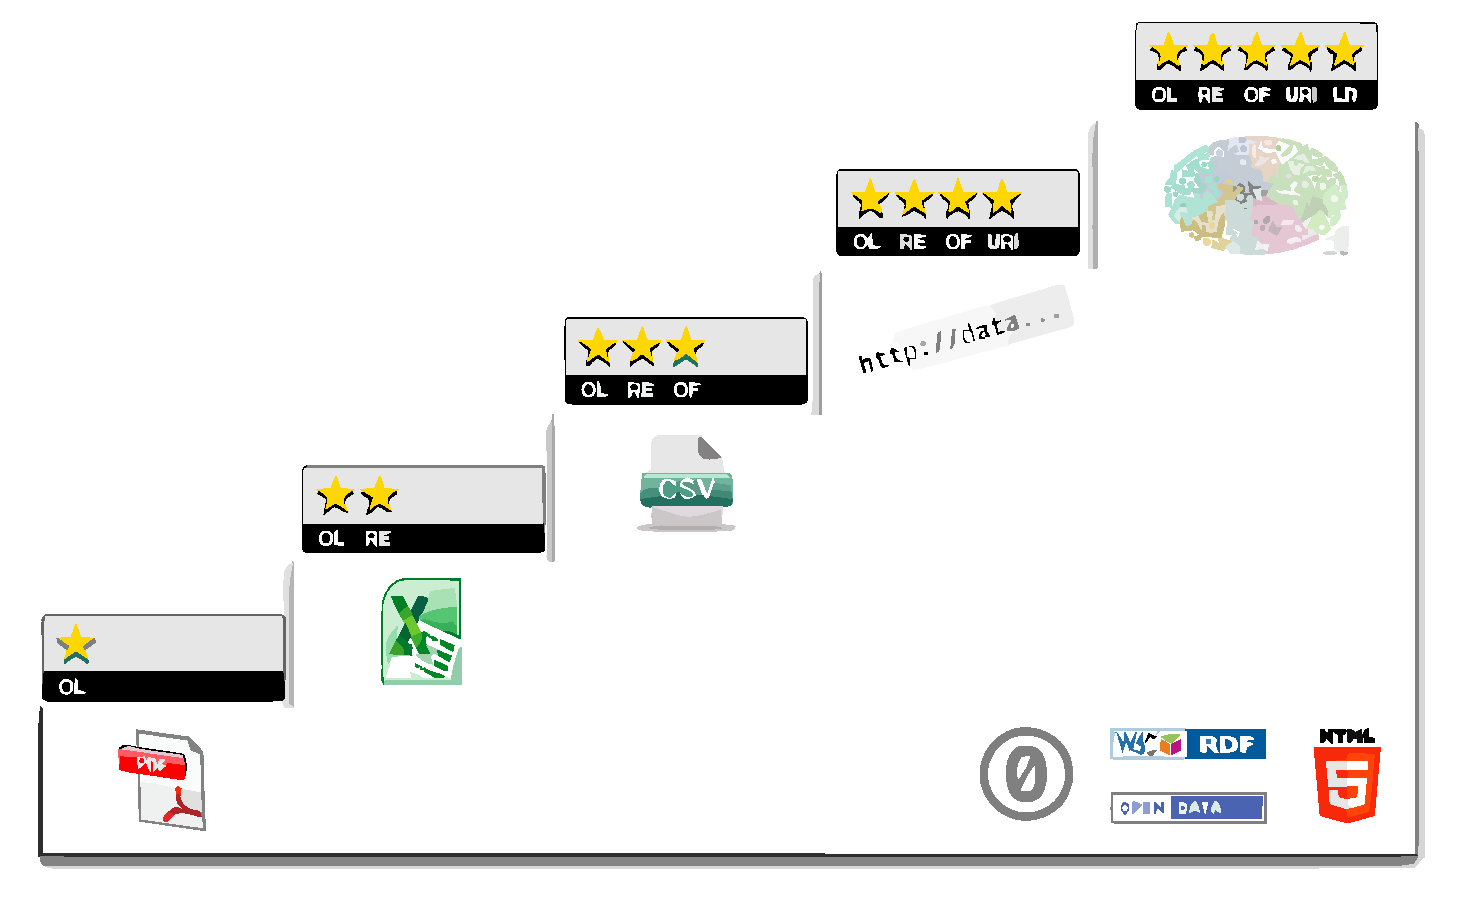
\includegraphics[scale=1.80]{img/5star-steps}
   \caption{Scala a 5 stelle}
   \label{fig:5star-steps}
\end{figure}

La scala a 5 stelle (fig. \ref{fig:5star-steps}) vuole misurare quanto i dati siano aperti e accessibili, assegnando le stelle secondo i seguenti criteri:

\begin{table}[htbp]
\begin{center}
\begin{tabularx}{\textwidth}{r X}
no star & \textbf{Web data} (in qualsiasi formato) senza nessuna licenza open\\
\ding{72} & Il dato � disponibile sul Web (in qualsiasi formato) con una \textbf{licenza aperta}\\
\ding{72} \ding{72} & Il dato � disponibile in un formato strutturato (ad esempio un Excel invece della scansione di una tabella) in modo che possa essere \textbf{riutilizzato}\\
\ding{72} \ding{72} \ding{72} & Il dato � in un \textbf{formato non proprietario} (ad esempio un CSV invece di un Excel)\\
\ding{72} \ding{72} \ding{72} \ding{72} & Il dato utilizza gli \textbf{URI} per identificare gli oggetti, in modo che le persone possano far riferimento alle sue risorse e fare uso di RDF\\
\ding{72} \ding{72} \ding{72} \ding{72} \ding{72} & Il \textbf{dato} � \textbf{collegato} ad altri dati per fornire un contesto\\
\end{tabularx}
\end{center}
\end{table} 

% Obama, ...
% \subsection{Open Data in ambito governativo}
Una grossa spinta all'affermazione del movimento Open Data in ambito governativo � stata data dal presidente degli Stati Uniti d'America \textbf{Barack Obama} con la promulgazione di una Direttiva sull'Open government nel dicembre 2009 \cite{Direttiva-OpenGovernament}:

\begin{quoting}
Fin dove possibile e sottostando alle sole restrizioni valide, le agenzie devono pubblicare le informazioni on line utilizzando un formato aperto (open) che possa cio� essere recuperato, soggetto ad azioni di download, indicizzato e ricercato attraverso le applicazioni di ricerca web pi� comunemente utilizzate. Per formato open si intende un formato indipendente rispetto alla piattaforma, leggibile dall�elaboratore e reso disponibile al pubblico senza che sia impedito il riuso dell�informazione veicolata.
\end{quoting}

Alla direttiva � stato dato seguito con la pubblicazione sul sito web \url{Data.gov} di molti dati in formato aperto. Il portale ha infatti lo scopo di raccogliere tutte le informazioni rese disponibili dagli enti statunitensi. \cite{wiki-datiaperti}
Nel maggio 2013 Barack Obama ha firmato un nuovo ordine esecutivo \cite{WhiteHouse-OpenData} che obbliga tutte le agenzie governative ad adottare dati in formato aperto compatibili anche con le future infrastrutture informatiche che verranno adottate negli USA. Le pubbliche amministrazioni dovranno assicurarsi, dove � legalmente consentito, che i dati vengano rilasciati in modo tale da risultare facilmente accessibili e utilizzabili.\\

% Italia
% \subsection{Open Data in Italia}
\textbf{In Italia} la spinta iniziale � stata data tra il 2007 e il 2010 dalla volont� di alcune amministrazioni locali che han voluto partecipare al progetto \href{http://www.openstreetmap.org/}{OpenStreetMap}, il quale crea e fornisce dati cartografici, come ad esempio mappe stradali, libere e gratuite a chiunque ne abbia bisogno.
I comuni coinvolti, insieme a dei volontari, hanno condiviso i dati dei propri stradari sotto licenza aperta.

Nel giugno 2010 Renato Brunetta, l'allora Ministro per la pubblica amministrazione e l'innovazione, dichiar� in un intervista l'intenzione di realizzare un portale italiano dell�Open data seguendo il modello dei datagov anglosassoni entro la fine dell'anno. Il 18 Ottobre 2011 il portale \url{dati.gov.it} � stato messo on line.

Nel maggio 2010 la regione Piemonte ha realizzato il proprio portale regionale \url{dati.piemonte.it}. Il sito � ancor oggi una delle esperienze nazionali con la miglior riuscita.
Nel 2011 la regione Emilia-Romagna ha seguito l'esempio piemontese.

A partire da settembre 2011 il Comune di Firenze, grazie anche alla spianta del suo Sindaco Matteo Renzi, ha realizzato il proprio portale \url{opendata.comune.fi.it} rilasciando un dataset al giorno nella fase iniziale. Inoltre Firenze � stato il primo comune a testare OpenBilancio, una visualizzazione dei dati che vuole essere comprensibile da tutti.

Nel marzo 2012 � stata rilasciata la seconda versione della licenza progettata per i dati delle Pubbliche Amministrazioni: Italian Open Data License, indicata come IODL v2.0 \cite{IODL2.0}, priva del vincolo "condividi-allo-stesso-modo" e con la sola richiesta di attribuzione della fonte per il riutilizzo dei dati. \cite{wiki-datiaperti}
	\section{Impianto Normativo}

Il percorso che ha portato all�attuale normativa in ambito Open Data � lungo e intreccia le sue radici con i concetti di \textit{libert� di informazione} e \textit{trasparenza della pubblica amministrazione} ed ha interessato i governi di differenti nazioni.

\begin{itemize}
\item 4 luglio 1966, viene emanato negli USA il \textbf{Freedom of Information Act} (FOIA) \cite{foia}, �atto per la libert� di informazione�, � una legge sulla libert� di informazione, che impone alle pubbliche amministrazioni una serie di regole per permettere a chiunque di sapere come opera il Governo federale.
Il FOIA ha aperto a giornalisti e studiosi l'accesso agli archivi di Stato statunitensi, a molti documenti riservati e coperti da segreto di Stato, di carattere storico o di attualit�. Il provvedimento � stato un punto importante per garantire la trasparenza della pubblica amministrazione nei confronti del cittadino, il diritto di cronaca e la libert� di stampa dei giornalisti.

%Rapporto Mandelkern:  D. Mandelkern,Diffusion des donn�es publiques et r�volution num�rique Commissariat g�n�ral du Plan, 1999 -> Dati pubblici essenziali

%Libro verde sull�informazione del settore pubblico nella societ� dell�informazione� della Commissione europea, 2000 

\item 24 novembre 2000, viene pubblicata nella Gazzetta Ufficiale le \textbf{Disposizioni per la delegificazione di norme e per la semplificazione di procedimenti amministrativi} (legge 340/2000) \cite{legge340/2000}
\begin{quoting}
Le pubbliche amministrazioni di cui all'articolo 1, comma 2, del decreto legislativo n. 29 del 1993 hanno accesso gratuito ai dati contenuti in pubblici registri, elenchi, atti o documenti da chiunque conoscibili.
\cite{legge340/2000}
\end{quoting}

%Data Quality Act � USA � 2001 (quality, objectivity, utility, and integrity of information)
	%https://en.wikipedia.org/wiki/Data_Quality_Act
	%http://rationalwiki.org/wiki/Data_Quality_Act
	%http://www.gpo.gov/fdsys/pkg/PLAW-106publ554/html/PLAW-106publ554.htm

\item 17 novembre 2003, viene approvata del Parlamento europeo e del Consiglio la \textbf{Direttiva relativa al riutilizzo dell�informazione del settore pubblico} (Direttiva PSI) \cite{direttiva-PSI} che incoraggia gli enti pubblici degli stati membri a massimizzare il potenziale dell'informazione rendendo disponibili e favorendo il riuso dei documenti, attraverso indici on line e licenze standard.

%Iniziative della Autorit� per la Informatica nella PA, anni 2000-2003.

\item 24 gennaio 2006, l�attuazione italiana della direttiva europea avviene con il \textbf{Decreto legislativo 24 gennaio 2006} \cite{decreto-legislativo2006}. Il provvedimento � stato predisposto dal Ministro per le politiche comunitarie e da quello per l'innovazione e le tecnologie, in accordo con i dicasteri degli Affari Esteri, Giustizia, Economia e Finanze, Funzione pubblica.
Esso definisce che il titolare del dato predispone le licenze standard per il riutilizzo e le rende disponibili, ove possibile in forma elettronica, sui propri siti istituzionali.
Gli Enti pubblici possono richiedere un compenso in denaro: in questo caso hanno l'obbligo di fissare e pubblicare le tariffe e le relative modalit� di versamento da corrispondere a fronte delle attivit�, individuandole sulla base dei costi effettivi sostenuti dalle Amministrazioni e aggiornato ogni due anni, comprende i costi di raccolta, di produzione, di riproduzione e diffusione maggiorati, nel caso di riutilizzo per fini commerciali.
� fatto divieto di esclusivit� sull�utilizzo dei dati.

%slides maurino parla di Nota 12 giugno 2008

\item 31 ottobre 2009, viene pubblicato in Gazzetta Ufficiale il Decreto legislativo n.150/2009, Attuazione della legge 4 marzo 2009, n. 15, in materia di \textbf{ottimizzazione della produttivit� del lavoro pubblico e di efficienza e trasparenza delle pubbliche amministrazioni} (legge Brunetta) \cite{legge-Brunetta}. IL Decreto indica le direttrici su cui articolare il riordino della pubblica amministrazione nella direzione della produttivit�, dell�efficienza e della trasparenza. Le direttrici individuate sono in particolare: il ciclo di gestione delle performance, la trasparenza e rendicontazione della perfomance, la misurazione e valutazione della perfomance, il merito, le nuove norme sull�ordinamento del lavoro pubblico ed il sistema sanzionatorio e disciplinare.

\item 22 giugno 2012, viene approvato il Decreto Legge \textbf{Misure urgenti per la crescita del Paese} (Decreto Sviluppo) \cite{decreto-sviluppo}.
\begin{quoting}
Art. 18
\begin{enumerate}
\item La concessione delle sovvenzioni, contributi, sussidi ed  ausili
finanziari alle imprese e  l'attribuzione  dei  corrispettivi  e  dei
compensi  a  persone,  professionisti,  imprese  ed  enti  privati  e
comunque  di  vantaggi  economici  di   qualunque   genere [...] ad enti pubblici  e
privati, sono soggetti alla pubblicit� sulla rete internet, ai sensi
del presente articolo e secondo il principio di accessibilit� totale [...]
\item Nei casi di cui  al  comma  1  ed  in  deroga  ad  ogni  diversa
disposizione di legge o  regolamento, nel  sito  internet  dell'ente
obbligato sono indicati:
\begin{enumerate}
\item il nome  dell'impresa  o  altro  soggetto
beneficiario ed i suoi dati fiscali;
\item l'importo;
\item la norma  o  il
titolo a base dell'attribuzione;
\item l'ufficio  e  il  funzionario  o
dirigente responsabile del relativo procedimento  amministrativo;
\item la modalit� seguita per l'individuazione  del  beneficiario;
\item il link al progetto selezionato, al curriculum del soggetto  incaricato,
nonch� al contratto e  capitolato  della  prestazione,  fornitura  o
servizio.
\end{enumerate}
\item Le informazioni [...] sono riportate, con  link  \emph{ben
visibile} nella homepage del sito, nell'ambito dei dati della  sezione
�Trasparenza,  valutazione  e  merito�  [...],  \emph{che  devono  essere  resi  di  facile
consultazione,  accessibili  ai  motori  di  ricerca  ed  in  formato
tabellare aperto che ne consente l'esportazione}, il trattamento e  il
riuso [...]
\item[5.] A decorrere dal 1� gennaio 2013, per le concessioni di  vantaggi
economici   successivi   all'entrata   in   vigore    del    presente
decreto-legge,  la  pubblicazione  ai  sensi  del  presente  \emph{articolo
costituisce condizione legale di efficacia  del  titolo}  legittimante
delle concessioni ed attribuzioni di importo complessivo \emph{superiore  a
mille euro nel corso dell'anno solare previste dal comma 1}, e la  sua
eventuale omissione  o  incompletezza  �  rilevata  d'ufficio  dagli
organi  dirigenziali  e  di  controllo,  \emph{sotto  la  propria   diretta
responsabilit� amministrativa,   patrimoniale   e   contabile}   per
l'indebita concessione o attribuzione  del  beneficio  economico. \emph{La
mancata, incompleta o ritardata pubblicazione � altres�  rilevabile
dal destinatario della  prevista  concessione  o  attribuzione  e  da
chiunque altro abbia interesse, anche ai fini}  del  risarcimento  del
danno  da   ritardo   da   parte   dell'amministrazione, [...]
\item[7.] Dall'attuazione del  presente  articolo  \emph{non  derivano  nuovi  o
maggiori oneri a carico  della  finanza  pubblica}  e  alle  attivit�
previste  \emph{si  far� fronte  con  le  risorse  umane,  finanziarie  e
strumentali disponibili a legislazione vigente}.
\cite{decreto-sviluppo}
\end{enumerate}
\end{quoting}
Con l�entrata in vigore di questo Decreto Legge inizia a prendere vita �Dentro il bilancio�, un progetto che amplia quello che precedentemente era \textit{OpenFatture}.





\end{itemize}









Articolo 52 cad 2012
%slides maurino (nuovo CAD)	
Il Codice dell'Amministrazione Digitale, all'art. 52, comma-1-bis, prevede che le Pubbliche Amministrazioni debbano promuovere "progetti di elaborazione e di diffusione dei dati pubblici di cui sono titolari", nonch� assicurarne la pubblicazione "in formati aperti", al fine di "valorizzare e rendere fruibili" i dati stessi.

Tale impostazione ha trovato autorevole conferma nel "Vademecum sull'OpenData" pubblicato dal Ministero per la Pubblica Amministrazione e l'Innovazione nel mese di ottobre 2011.
http://www.dati.gov.it/sites/default/files/VademecumOpenData.pdf


Open data by default 2012
% forse 2013
%Slides maurino Open data by default

%http://www.morenaragone.it/?p=316
	%decreto-legge 22 giugno 2012, n. 83
	%decreto-legge 12 ottobre 2012, n. 179
	%legge 6 novembre 2012, n. 190

%Con l'entrata in vigore del D.Lgs. n. 33 /2013 "Riordino della disciplina riguardante gli obblighi di pubblicit�, trasparenza e diffusione di informazioni da parte delle pubbliche amministrazioni", l�Amministrazione comunale sta provvedendo all�adeguamento delle pagine del sito web.


% 5o7 giugno direttiva PSI


%leggi regionali...
	%http://www.dati.piemonte.it/novita/1-ultime/875-la-nuova-direttiva-europea-in-materia-di-psi.html
\newpage %nuova pagina

%-------------------------------------------------------------------------

\chapter{Piattaforme Tecnologiche} 
	\section{Socrata (Open Source)}
% Versione Open Source
Socrata � una piattaforma sviluppata dall'omonimia societ� con sede negli Stati Uniti d'America. Socrata � un servizio "Software as a service".
Dal 10 aprile 2013 � disponibile anche in una versione Community Edition rilasciata come Open Source al fine di promuovere uno standard intorno ai dati aperti e far crescere la comunit�.

Il Socrata Open Data Server e le componenti che lo compongono sono stati resi disponibili con licenza Apache. 
L�architettura del sistema pu� quindi essere suddivisa in una serie di componenti separate che la compongono come mostrato in figura \ref{fig:socrata-architecture}.

\begin{figure}[htbp]
   \centering
   \includegraphics[scale=0.55]{img/socrata-architecture.jpg}
   \caption{Architettura di Socrata}
   \label{fig:socrata-architecture}
\end{figure}

SODA 2 fornisce quindi l�accesso ai dati puri attraverso SoQL (SODA Query Language) e delle semplici API per aggiornarli.
La scrittura avviene quindi attraverso un percorso che prevede il seguente percorso:
\begin{enumerate}
\item[\textcolor{Orange}{\ding{202}}] Un�applicazione o un processo inizia un�operazione sul SODA Server.
\item[\textcolor{Orange}{\ding{203}}] La richiesta viene trasformata in una serie di operazioni pi� elementari chiamante �mutations� e vengono passate al Data Coordinator in modo da essere eseguite sul database (Postgres).
\item[\textcolor{Orange}{\ding{204}}] Dopo che il Data Coordinator ha finito, il Secondary Watcher si sveglia e guarda se ci sono cambiamenti nel database che non sono ancora stati sincronizzati.
\item[\textcolor{Orange}{\ding{205}}] L�adattatore per l�archivio secondario (in questo caso Elastic Search) importa i dati dal primario.
Ci� permette in caso di guasti di re-sincronizzare il database.
\end{enumerate}

Mentre la lettura avviene attraverso:
\begin{enumerate}
\item[{\includegraphics[scale=0.028]{img/A}}] Un�applicazione invia una richiesta al server SoQL. Questa viene analizzata come descritto serctitto in soql-reference.
\item[{\includegraphics[scale=0.028]{img/B}}] Il Query Coordinator determina a quale database inviare la richiesta (in futuro ci portano essere diversi archivi secondari).
\item[{\includegraphics[scale=0.028]{img/C}}] Il Query Coordinator passa fuori la query all�adattatore appropriato che esegue la query sull�archivio corretto e restituisce l'appropriato payload C-JSON.
\end{enumerate}

Ad oggi sono state rese disponibili con licenza Open Source solo alcune parti:

\begin{itemize}
\item \textbf{soql-reference}, Implementazione di riferimento del linguaggio di interrogazione SoQL.
\item \textbf{socrata-http}, Toolkit per la creazione di servizi HTTP.
\item \textbf{soql-es-adapter}, ElasticSearch Secondary Store per SoQL Data Service.
\item \textbf{socrata-csv}, Un sottile involucro Scalaish intorno ad opencsv.
\item \textbf{socrata-utils}, Classi-Utility utilizzate in tutto il Socrata Open Data Server.
\item \textbf{data-coordinator}, Coordina la distribuzione degli aggiornamenti tra archivi di dati primari e secondari.
\end{itemize}

La Community Edition condivide lo stesso core della versione proprietaria, ma al momento manca completamente il front-end per gestire comodamente i dataset che � invece presente nella versione SaaS.
Secondo la Roadmap intorno all'Agosto 2013 era previsto il rilascio della versione beta finale, compresa della documentazione e degli strumenti che avrebbero permesso di installare e rendere funzionate l'intero Open Data Server.

Socrata offre sia numerose API per gestire i dataset, che strumenti di visualizzazione che mostrano i dati caricati attraverso un sistema di preview tabellare dotato di filtri avanzati, oppure su diverse tipologie di mappe in caso di dati geolocalizzati.
Permette inoltre di esportare i dati in vari formati (CSV, XLS, XLSX, XML, JSON).

In Italia Socrata � stata usata con successo dalla Regione Lombardia con un centinaio di dataset pubblicati.
	\section{CKAN}
CKAN (Comprehensive Knowledge Archive Network) � un potente sistema DMS (Data Management System) open source, ovvero un sistema di gestione dei dati. Esso ha lo scopo di renderli accessibili permettendo la loro archiviazione e distribuzione attraverso una comoda interfaccia web che semplifica la pubblicazione, la condivisione, la ricerca e l'utilizzo dei dati.
Inoltre CKAN offre numerose API per gestire i dataset e strumenti di visualizzazione che permettono un anteprima, siano essi semplici tabelle o dati geolocalizzati.

CKAN � rivolto ai data publishers, siano essi governi, imprese o organizzazioni nazionali/regionali, che vogliono fare i loro renderli disponibili i loro dati e renderli facilmente fruibili.

Il suo codice � mantenuto dalla Open Knowledge Foundation ed � utilizzato come piattaforma per gestire cataloghi pubblici da siti come \url{thedatahub.org}, \url{catalog.data.gov}, \url{data.gov.uk} e \url{PublicData.eu}.
	\input{3.Piattaforme-Tecnologiche/3.Sister.it}
\newpage %nuova pagina

%-------------------------------------------------------------------------

\chapter{Progettazione portale OpenData a Vigevano} 
	\section{Descrizione del Comune}
% Storia
La citt� di Vigevano si trova a 30 chilometri da Milano, tra i boschi del Ticino. 

%-------------
Circondata dai boschi del Parco del Ticino, a soli 30 chilometri da Milano, Vigevano accoglie il visitatore con l'armonia della celebre Piazza Ducale: \"{}una sinfonia su quattro lati\"{} secondo la definizione del grande maestro Arturo Toscanini.

Ideata dal Bramante con il concorso di Leonardo da Vinci, Piazza Ducale � l'ingresso d'onore all'imponente Castello, per estensione uno dei pi� grandi d'Europa e in fase avanzata di restauro e di riuso grazie all'organizzazione di mostre e alla prossima apertura di musei.

Citt� d'arte ma anche citt� d'acque, Vigevano � attraversata da canali e dal fiume Ticino che offre scorci e oasi naturali di indubbio fascino.

Da Ludovico il Moro a Eleonora Duse, allo scrittore Lucio Mastronardi, sono tanti i personaggi che hanno visto la luce in una citt�, ancora oggi nota in tutto il mondo per la produzione di scarpe di qualit� e per la sua industria meccano-calzaturiera.

\subsection{Origini}
Di origine longobarda Vigevano nasce come luogo fortificato corrispondente all'attuale cortile del Castello. Successivamente si sviluppa il borgo esterno, le cui case ed edifici sorgono sul luogo oggi occupato dalla famosa Piazza Ducale.

Si trasforma in libero Comune a partire dal 1198, mentre nel 1277 la storia di Vigevano si lega a quella delle potenti famiglie milanesi dei Visconti prima e degli Sforza poi.

Grazie all'opera di Luchino Visconti e di Ludovico Sforza detto il Moro, tra XIV e XV secolo, il borgo di Vigevano inizia la sua trasformazione in residenza estiva, in delizioso soggiorno per gli svaghi e gli ozi della corte ducale: il Castello viene adibito a dimora di prestigio grazie all'opera di artisti come Bramante, la Piazza Ducale in scenografico spazio libero da case ed edifici, regale atrio d'ingresso al Castello

Nel 1530 Vigevano ottiene il titolo di citt� con una propria sede vescovile.



%- Organizzativo sistemi informativi
%Dovrebbe essere sul loro sito

	\section{Progettazione piattaforma}
%a partire dal git in automatico su ckan con metadati
%\begin{quoting}
Con delibera 14 del 19/01/2012 il Comune di Vigevano, nell'ambito del Progetto InnoVi, cofinanziato dalla regione, ha adottato, in riuso dal Comune di Milano, la piattaforma \textbf{GIT}, un integratore di banche dati interne ed esterne all'ente e relativa cartografia, con il project management di Ancitel Lombardia ed il supporto tecnico della societ� HiWeb Srl della Regione Umbria che ha contribuito a far nascere e crescere tale sistema.
%[...]
Il sistema GIT � un ricco contenitore di informazioni alfanumeriche e grafiche correlate, periodicamente aggiornate, e che, per questo, � un candidato naturale ad alimentare dei dataset di dati da rendere disponibili con licenze open, opportunamente filtrati ed aggregati allo scopo di tutelare la privacy.
\cite{CittaVigevano-GCn104}
%\end{quoting}
Vogliamo quindi una piattaforma che permetta di integrare le informazioni presenti sulla piattaforma GIT con il portale Open Data che verr� realizzato.
Per fare ci� sono percorribili tre strade distinte:
\begin{enumerate}
\item Effettuare periodicamente delle esportazioni dei dati da GIT per caricarle sulla piattaforma.
\item Effettuare l'aggiornamento dei dati sulla piattaforma ogni volta che vengono aggiornati su GIT in automatico.
\item Permettere alla piattaforma di accedere direttamente ai dati di GIT.
\end{enumerate}

La terza soluzione presenta dei problemi di sicurezza, perch� per realizzarla bisogna modificare GIT creando un interfaccia che permetta l'interrogazione ai dati dall'esterno. Ci� pu� diventare un problema nel momento in cui si creano delle API di interrogazioni generiche e quindi in alcune occasioni si finisce a violare la privacy degli utenti.

La prima soluzione pu� essere applicata nei casi in cui le informazioni hanno una frequenza di aggiornamento rada, ma diventa impraticabile nel momento in cui i dati vengo aggiornati con una frequenza rilevante, in quando bisogna fare manualmente un aggiornamento ogni volta.

La soluzione vincente risulta quindi essere la seconda, essa comporta un controllo degli eventi sulla piattaforma GIT e l'esistenza di un sistema di aggiornamento automatizzato (senza intervento umano) sulla piattaforma Open Data.
Nell'ottica del riutilizzo del software, questa componente deve essere in grandi di controllare eventuali aggiornamenti di GIT, di anonimizzare i dati e di inserirli nella piattaforma attraverso API.\\

%Catalogo e dizionario
Al fine di agevolare l'integrazione tra la piattaforma e applicazioni di terze parti si vuole rendere disponibile un \textbf{catalogo} contenente tutti i dataset e i relativi metadati. Con Metadati si intendono le informazioni riguardanti il singolo dataset quali il suo nome, la sua descrizione, il formato del file, la sua data di ultima modifica, il link a cui raggiungere la risorsa, ...

Si vuole inoltre rendere disponibile per ogni dataset il dizionario dei dati in esso contenuto. Ci� vuol dire che nel catalogo sar� presente anche l'informazione della tabella per ogni singolo dataset.

In questo modo � possibile interrogare il dataset sapendo a priori il tipo di dato che � contenuto in esso.\\

%Triggher e workflow
Si � scelto di utilizzare una piattaforma open source in accordo con il Comune di Vigevano e di conseguenza CKAN � stata la piattaforma sulla quale si � scelto di implementare i requisiti.
Al fine di rendere compatibile le modifiche apportate alla piattaforma CKAN tra le varie versioni della stessa si � deciso di analizzarlo come una �scatola nera�, senza mettere mano al codice sorgente di CKAN.

\begin{figure}[htbp]
   \centering
   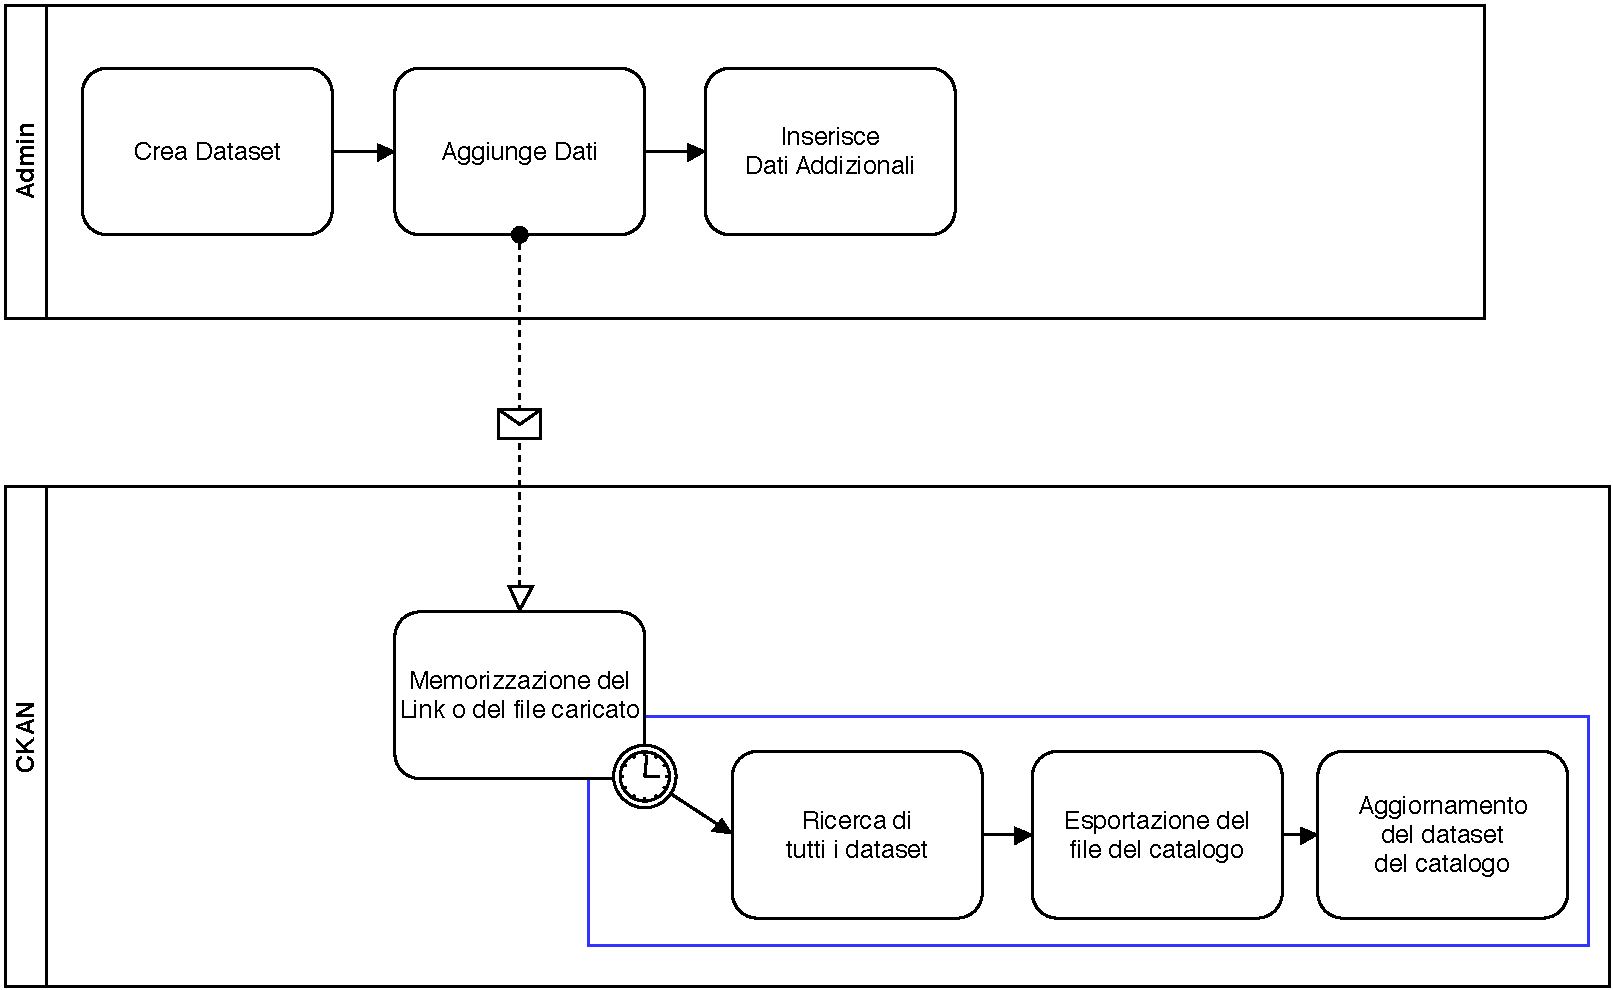
\includegraphics[scale=0.5]{img/workflow-creazione-dataset} % requires the graphicx package
   \caption{Workflow dell�aggiornamento del catalogo al momento dell�inserimento di un nuovo dataset}
   \label{fig:workflow}
\end{figure}

La progettazione del catalogo � quindi stata fatta come mostrato in fig. \ref{fig:workflow} inserendo un triggher (una procedura che viene eseguita in maniera automatica in coincidenza di un determinato evento) che ad ogni aggiornamento nel database della tabella contenente i dataset venga fatta una query che restituisce il catalogo (facendo un join tra diverse tabelle) e la esporti in formato CSV. Il file contenete il catalogo � esso stesso parte integrante della piattaforma essendo a sua volta un dataset.

	\section{Integrazione con Regione Lombardia}

Lorem ipsum dolor sit amet, consectetur adipiscing elit. Nulla lacinia diam id commodo dignissim. Curabitur feugiat id est a pellentesque. Ut varius vel nisi vitae scelerisque. Aliquam faucibus blandit arcu, id fermentum elit placerat a. Donec a lacinia lectus. Nullam id blandit ante. Cras a dui pharetra, fermentum velit at, laoreet elit. Vestibulum justo lectus, tempor imperdiet cursus vitae, lobortis eu mauris. Nunc lacinia pretium dui blandit sagittis. Maecenas eget purus eros. Nam tortor sapien, pellentesque nec lectus quis, egestas consequat tortor.

Duis a risus ut nulla ullamcorper interdum eu quis dolor. Aliquam pretium rhoncus libero vitae venenatis. Vestibulum vulputate purus vel gravida viverra. Mauris metus felis, dignissim sed suscipit ut, tincidunt eget neque. Etiam et mi ultrices, porta odio at, rutrum lorem. Phasellus posuere tellus quis justo semper, non eleifend felis viverra. Suspendisse blandit luctus dui, et mollis nulla molestie eget. Cras mattis, quam ac pulvinar tristique, nibh nisi scelerisque neque, vitae egestas massa tortor sed nibh. Interdum et malesuada fames ac ante ipsum primis in faucibus. Proin convallis velit nec nisl laoreet sagittis. Nam arcu ipsum, vehicula a feugiat vel, dictum sit amet sapien. Cras sit amet eros sed eros eleifend vulputate a laoreet lacus. Nullam pulvinar enim at massa cursus, sed adipiscing tortor tristique. Phasellus et neque in nisi blandit sodales.

Cras ac sapien ipsum. Integer consectetur, lectus vitae semper bibendum, urna magna tempor tortor, sit amet accumsan libero diam ut odio. Cras ut facilisis lectus, at fringilla erat. Pellentesque non luctus purus. Aenean urna metus, facilisis id adipiscing fermentum, porta faucibus lacus. Sed vitae nulla viverra, egestas turpis eu, eleifend quam. Interdum et malesuada fames ac ante ipsum primis in faucibus. In a lacus enim.

Vivamus imperdiet id erat ut pulvinar. Phasellus vel gravida dolor. Morbi augue odio, sollicitudin id porttitor quis, tincidunt id orci. Mauris mollis, nisl vitae pretium lacinia, purus mauris euismod elit, a vulputate eros ipsum ut dolor. Nam eu tristique mauris. Quisque orci dui, feugiat a vestibulum non, convallis id justo. Mauris vestibulum mauris sed placerat elementum. In id orci augue. 
\newpage %nuova pagina

%-------------------------------------------------------------------------

\chapter{Sviluppo della soluzione} 
	\input{5.Sviluppo-della-soluzione/1.Caricamento-automatico}
	%\section{Dizionario dati}
\section{Catalogo dati}

Una volta che CKAN � stato popolato di dataset si � realizzato il catalogo dei dataset presenti.
Per fare ci� � stato necessario recuperare le informazioni contenute nel database e quindi le tabelle prese in esame sono state \texttt{package}, \texttt{resource} e \texttt{resource\_group}. La loro struttura � mostrata in figura \ref{fig:DB-design}:

\begin{figure}[htbp]
   \centering
   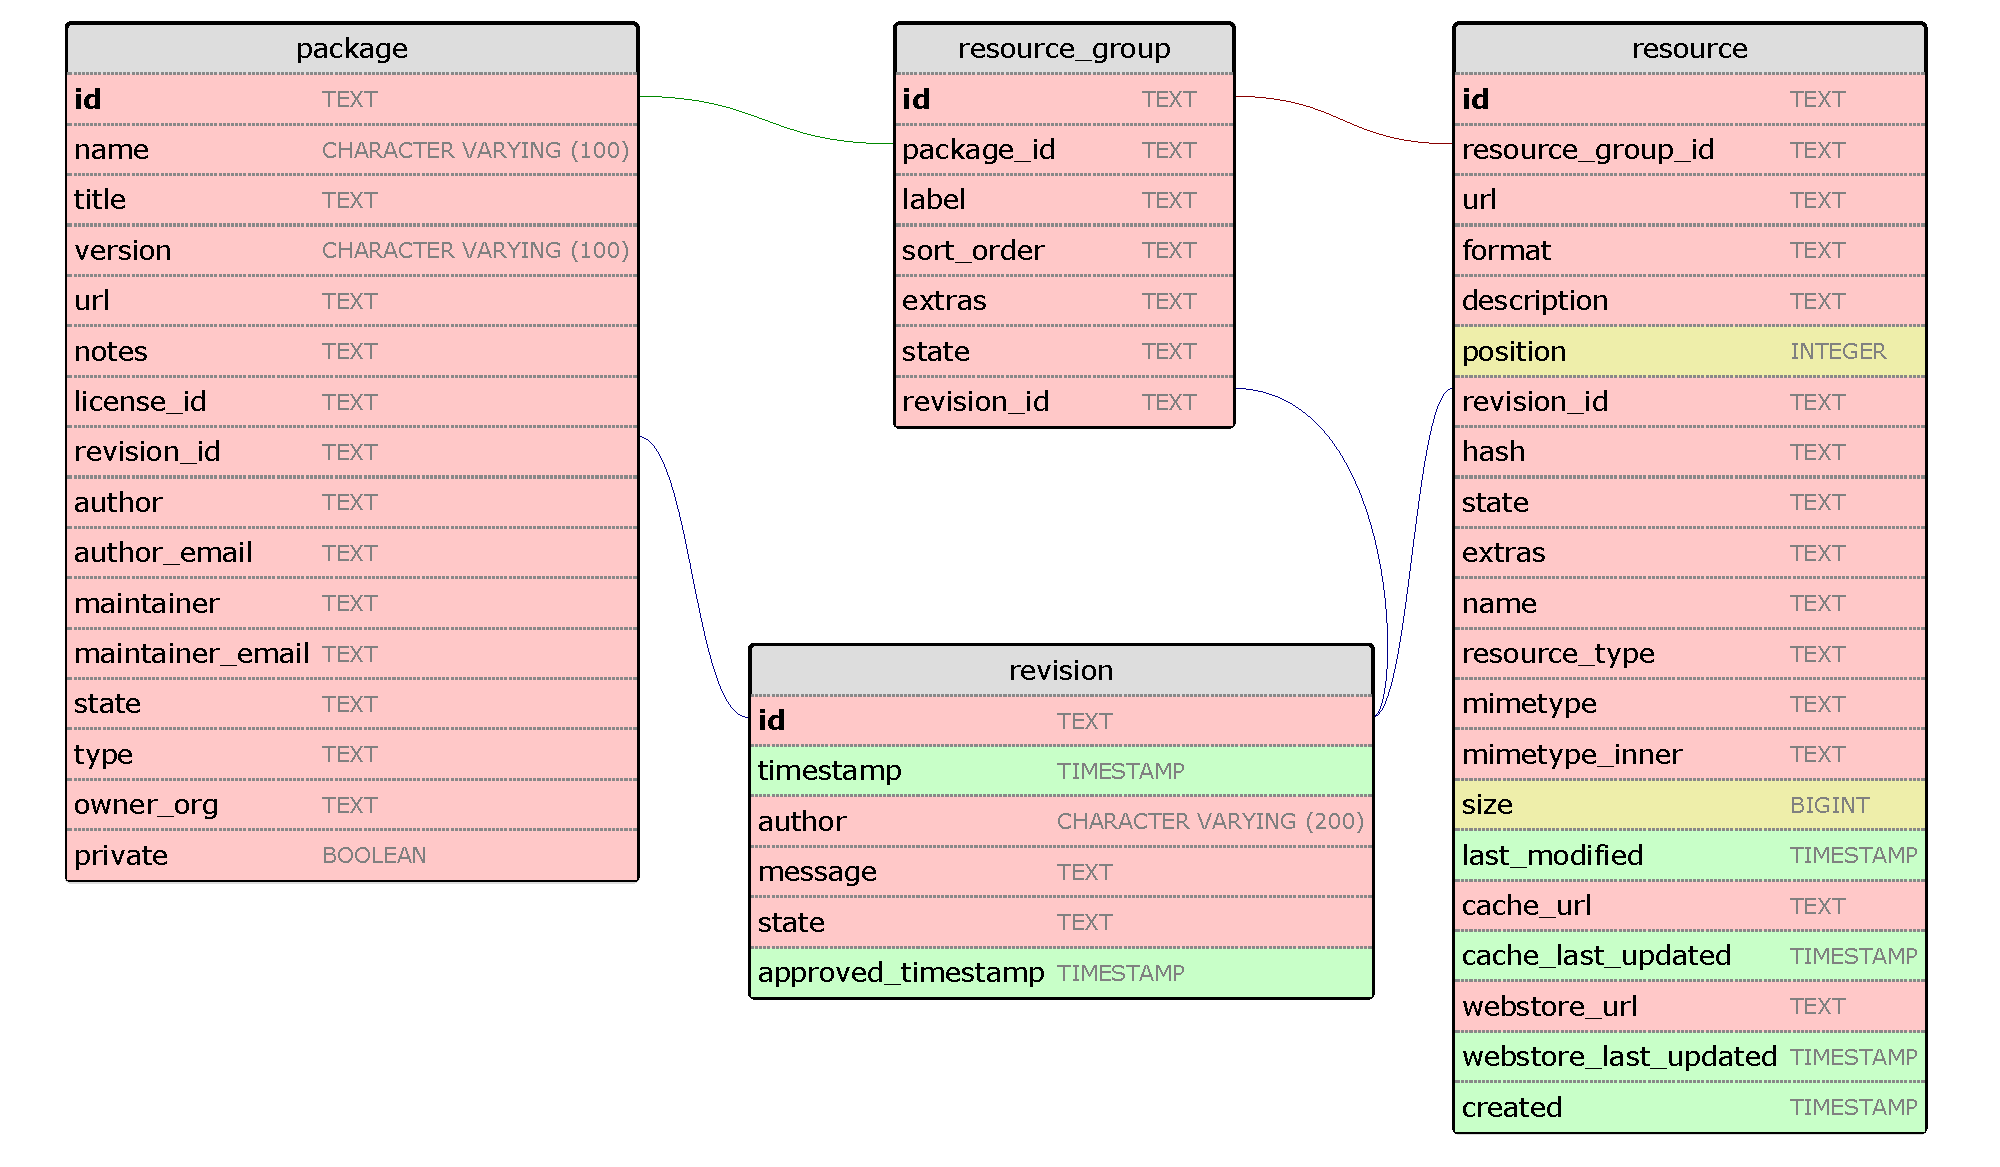
\includegraphics[scale=0.40]{img/DB-design2}
   \caption{Design DataBase}
   \label{fig:DB-design}
\end{figure}

Le informazioni sono presenti in tabelle differenti, ed � quindi stato necessario fare un JOIN tra le 3 tabelle e successivamente selezionare solo i campi di nostro interesse. Inoltre si sono tradotte le intestazioni delle colonne in italiano e si � creato un nuovo campo (link) concatenando l�url base della piattaforma con le informazioni presenti nel database.
%Per realizzare tutto ci� si � utilizzato la seguente query:\\
%{\indent{\footnotesize \verb$SELECT "name" AS "nome", "description" AS "descrizione", "url" AS "url",$}}\\
%{\indent{\footnotesize \verb$ "format" AS "formato", "last_modified" AS "ultima modifica",$}}\\
%{\indent{\footnotesize \verb$ "author" AS "autore", "author_email" AS "email autore",$}}\\
%{\indent{\footnotesize \verb$ "maintainer" AS "manutentore", "maintainer_email" AS "email manutentore",$}}\\
%{\indent{\footnotesize \verb$ CONCAT('http://localhost/dataset/',url_name,'/resource/',url_id) AS "link"$}}\\
%{\indent{\footnotesize \verb$FROM	($}}\\
%{\indent{\footnotesize \verb$ SELECT	"name", "description", "url", "format", "last_modified",$}}\\
%{\indent{\footnotesize \verb$   "resource_group_id", "package_id", resource.id AS "url_id"$}}\\
%{\indent{\footnotesize \verb$ FROM	"resource_group"$}}\\
%{\indent{\footnotesize \verb$ JOIN	"resource"$}}\\
%{\indent{\footnotesize \verb$ ON	resource_group.id=resource.resource_group_id$}}\\
%{\indent{\footnotesize \verb$ WHERE	"name"<>'datacatalog.csv'$}}\\
%{\indent{\footnotesize \verb$ ) AS "resource"$}}\\
%{\indent{\footnotesize \verb$JOIN	($}}\\
%{\indent{\footnotesize \verb$ SELECT	"id", "author", "author_email", "maintainer", "maintainer_email",$}}\\
%{\indent{\footnotesize \verb$  "name" AS "url_name"$}}\\
%{\indent{\footnotesize \verb$ FROM	"package") AS "package"$}}\\
%{\indent{\footnotesize \verb$ON	resource.package_id=package.id$}}\\
%{\indent{\footnotesize \verb$ORDER BY "last_modified" DESC;$}}\\

Ci� � stato realizzato attraverso una query, il cui risultato � stato esportato in un file in formato CSV (comma-separated values). Si � voluto salvare il file in una posizione che fosse poi recuperabile dal web server, di conseguenza si � scelto di salvarlo nella sua root. Ci� � possibile utilizzando il comando \textit{Copy} dopo aver acceduto al database PostgreSQL:\\

\shellcmd{sudo psql -h localhost -U ckanuser ckan\_default}
{\indent\indent{\footnotesize \verb$\Copy ($}}\\
\\
\centerline{\texttt{...QUERY...}}\\
\\
{\indent\indent{\footnotesize \verb$) To '/usr/lib/ckan/default/src/ckan/ckan/public/datacatalog.csv'$}}\\
{\indent\indent{\footnotesize \verb$With CSV HEADER$}}\\

  
Successivamente, per automatizzare il processo di creazione del catalogo ad ogni nuovo inserimento di un dataset in CKAN, sono stati creati una funzione ed un trigger.

Per fare ci� si accede a postreSQL e si assegnano i permessi di SuperUser all�utente utilizzato per creare il database:\\

\shellcmd{sudo -u postgres psql}
{\indent\indent{\footnotesize \texttt{\footnotesize\textcolor{NavyBlue}{=\#}} \verb#alter role ckanuser SUPERUSER;#}}\\

Ci� � necessario affinch� la funzione che andiamo a creare possa esportare il database all�esterno dell�ambiente.
Accediamo quindi al database e procediamo con la creazione di funzione e trigger:\\

\shellcmd{sudo psql -h localhost -U ckanuser ckan\_default}

La funzione non fa altro che eseguire l'esportazione della query in CSV nella posizione prestabilita:\\

{\indent{\footnotesize \verb#CREATE FUNCTION create_datacatalog ()#}}\\
{\indent{\footnotesize \verb#RETURNS trigger#}}\\
{\indent{\footnotesize \verb#AS $create_datacatalog$#}}\\
{\indent{\footnotesize \verb#BEGIN EXECUTE '#}}\\
{\indent{\footnotesize \verb#Copy (SELECT "name" AS "nome", "description" AS "descrizione", "url" AS#}}\\
{\indent{\footnotesize \verb# "url", "format" AS "formato", "last_modified" AS "ultima modifica",#}}\\
{\indent{\footnotesize \verb# "author" AS "autore", "author_email" AS "email autore", "maintainer"#}}\\
{\indent{\footnotesize \verb# AS "manutentore", "maintainer_email" AS "email manutentore" FROM (#}}\\
{\indent{\footnotesize \verb# SELECT "name", "description", "url", "format", "last_modified",#}}\\
{\indent{\footnotesize \verb# "resource_group_id", "package_id", resource.id AS "url_id"#}}\\
{\indent{\footnotesize \verb# FROM "resource_group" JOIN "resource"#}}\\
{\indent{\footnotesize \verb# ON resource_group.id=resource.resource_group_id) AS "resource"#}}\\
{\indent{\footnotesize \verb# JOIN (SELECT "id", "author", "author_email", "maintainer",#}}\\
{\indent{\footnotesize \verb# "maintainer_email", "name" AS "url_name" FROM "package") AS "package"#}}\\
{\indent{\footnotesize \verb# ON resource.package_id=package.id ORDER BY "last_modified" DESC)#}}\\
{\indent{\footnotesize \verb# To ''/usr/lib/ckan/default/src/ckan/ckan/public/datacatalog.csv''#}}\\
{\indent{\footnotesize \verb# With CSV HEADER;#}}\\
{\indent{\footnotesize \verb#';#}}\\
{\indent{\footnotesize \verb#RETURN NEW;#}}\\
{\indent{\footnotesize \verb#END;#}}\\
{\indent{\footnotesize \verb#$create_datacatalog$#}}\\
{\indent{\footnotesize \verb#LANGUAGE plpgsql;#}}\\
\\
Mentre invece il trigger si attiva ad ogni modifica della tabella \texttt{resource} e invoca la funzione:\\

{\indent{\footnotesize \verb#CREATE TRIGGER datacatalog_update#}}\\
{\indent{\footnotesize \verb#AFTER insert OR update#}}\\
{\indent{\footnotesize \verb#ON resource#}}\\
{\indent{\footnotesize \verb#FOR EACH ROW#}}\\
{\indent{\footnotesize \verb#EXECUTE PROCEDURE create_datacatalog();#}}\\
\\

Infine per rendere possibile la modifica del file \texttt{datacatalog.csv} da parte del web server si `e assegnato al file i permessi di scrittura all�utente \texttt{postgresql}:\\

\shellcmd{sudo touch /usr/lib/ckan/default/src/ckan/ckan/public/datacatalog.csv}
\shellcmd{sudo chmod 644 /usr/lib/ckan/default/src/ckan/ckan/public/datacatalog.csv}
\shellcmd{sudo chown postgres:postgres /usr/lib/ckan/default/src/ckan/ckan\\/public/datacatalog.csv}


\section{Dizionario dati}
Nelle intenzioni dello sviluppo della piattaforma si � cercato di aggiungere nel catalogo anche le informazioni sul tipo di dato contenuto in ogni singolo dataset. In pratica si voleva inserire un�ulteriore colonna nel catalogo contenente le intestazioni della tabella del dataset.
Purtroppo non si � trovata una soluzione per realizzare questa feature in quanto non si � trovato il modo di recuperare le informazioni presenti nei due differenti database che sono relazionati come mostrato in figura \ref{fig:DBs-ckan}.%:

\newpage
\begin{figure}[htbp]
   \centering
   \includegraphics[scale=0.48]{img/DBs-ckan_clear.png}
   \caption{relazione tra le tabelle dei DataBase utilizzati da CKAN}
   \label{fig:DBs-ckan}
\end{figure}

L�impossibilit� di recuperare l�intestazione delle tabelle del database \texttt{datastore\_default} una volta conosciuto il valore nel campo \texttt{id} dei singoli elementi presenti nella tabella \texttt{resource} del database \texttt{ckan\_default} non ha quindi al momento permesso la creazione del dizionario dati.
	\section{Blueprint}

Per realizzare l�integrazione tra la piattaforma CKAN realizzata per il Comune di Vigevano e la piattaforma Socrata utilizzata da Regione Lombardia si � pensato di importare il catalogo della prima nella seconda.\\

Dalla documentazione presente su Socrata si � ipotizzato di utilizzare quanto descritto alla pagina \url{http://dev.socrata.com/publishers/importing}.

L�importazione dei dati viene eseguita come un processo in due fasi. In primo luogo, il file di dati in s� viene caricato tramite l'API, e viene poi analizzato per determinare il tipo di dati che esso contiene. I risultati di tale analisi vengono restituiti, dopodich� � possibile apportare modifiche al modo in cui l'importatore interpreta i dati. A questo punto si invia il progetto di importazione risultante, e a questo punto inizia il processo di importazione vero e proprio.

Al momento questa soluzione non � stata ancora sperimentata, mancando i tempi tecnici di realizzazione.
\newpage %nuova pagina

%-------------------------------------------------------------------------

\chapter{Utilizzo della piattaforma}

Dopo la prima installazione la piattaforma si presenta, come mostrato in figura \ref{fig:demo-1-ckan-vergine}, con un�interfaccia sobria e  pronta a contenere i dataset che varranno caricati.

\begin{figure}[htbp]
   \centering
   \includegraphics[scale=0.42]{img/demo-1-ckan-vergine}
   \caption{Aspetto di CKAN appena installato}
   \label{fig:demo-1-ckan-vergine}
\end{figure}

\newpage
Navigando alla voce di men� �Dataset� � possibile vedere l�elenco dei dataset disponibili, ma anche crearne uno nuovo attraverso il pulsante presente in alto a destra (figura \ref{fig:demo-2-ckan-creazione-dataset}).

\begin{figure}[htbp]
   \centering
   \includegraphics[scale=0.42]{img/demo-2-ckan-creazione-dataset}
   \caption{Elenco dei Dataset vuoto}
   \label{fig:demo-2-ckan-creazione-dataset}
\end{figure}

\newpage
L�inserimento di un nuovo Dataset inizia con la richiesta di inserimento delle meta-informazioni necessarie alla sua identificazione (figura \ref{fig:demo-3-ckan-primo-passo}), ovvero il titolo e la descrizione; l�utente pu� anche decidere di inserire opzionalmente alcuni tag per facilitarne la ricerca e la licenza da un elenco predefinito.

\begin{figure}[htbp]
   \centering
   \includegraphics[scale=0.42]{img/demo-3-ckan-primo-passo}
   \caption{Definizione dei metadati durante la creazione di un dataset}
   \label{fig:demo-3-ckan-primo-passo}
\end{figure}

\newpage
Ad esempio possiamo inseriti i metadati necessari alla creazione del catalogo (figura \ref{fig:demo-3-ckan-primo-passo-condati}) per poi passare all�aggiunta dei dati veri e prorpi.

\begin{figure}[htbp]
   \centering
   \includegraphics[scale=0.42]{img/demo-3-ckan-primo-passo-condati}
   \caption{Inserimento metadati del catalogo}
   \label{fig:demo-3-ckan-primo-passo-condati}
\end{figure}

\newpage
Nel secondo passaggio � possibile linkare un file o una risorsa esterna e specificare il nome e la descrizione che verranno utilizzati nella piattaforma (figura \ref{fig:demo-4-ckan-secondo-passo-condati}). Il formato del file viene identificato automaticamente, in caso ci� non avvenga � possibile inserirlo manualmente.

\begin{figure}[htbp]
   \centering
   \includegraphics[scale=0.42]{img/demo-4-ckan-secondo-passo-condati}
   \caption{Inserimento risorsa nel dataset}
   \label{fig:demo-4-ckan-secondo-passo-condati}
\end{figure}

\newpage
In alternativa, una volta attivato il File Store � possibile caricare un file dal proprio computer in modo che venga memorizzato nel server (figura \ref{fig:demo-7-upload-scuola}). Un messaggio ci avvertir� del successo dell�upload o dell�eventuale fallimento nella parte alta dello schermo.

\begin{figure}[htbp]
   \centering
   \includegraphics[scale=0.42]{img/demo-7-upload-scuola}
   \caption{Upload fine in CKAN}
   \label{fig:demo-7-upload-scuola}
\end{figure}

\newpage
Infine � possibile aggiungere ulteriori informazioni riguardanti l�autore dei dati e il manutentore (colui che si preoccupa di aggiornare il dataset nel tempo). Inoltre � possibile assegnare in dataset ad un gruppo (figura \ref{fig:demo-5-ckan-terzo-passo-condati}).

\begin{figure}[htbp]
   \centering
   \includegraphics[scale=0.42]{img/demo-5-ckan-terzo-passo-condati}
   \caption{Inserimento dati addizionali del dataset}
   \label{fig:demo-5-ckan-terzo-passo-condati}
\end{figure}

\newpage
A questo punto ci viene mostrato il dataset con tutte le informazioni che abbiamo inserito (figura \ref{fig:demo-6-ckan-catalogo-vuoto}). Finch� il DataStorer non entra in funzione la preview non sar� disponibile.

\begin{figure}[htbp]
   \centering
   \includegraphics[scale=0.42]{img/demo-6-ckan-catalogo-vuoto}
   \caption{Dataset appena caricato, il DataStorer non � ancora entrato in funzione}
   \label{fig:demo-6-ckan-catalogo-vuoto}
\end{figure}

\newpage
Una volta che il file sar� processato e i dati contenuti nel dataset saranno salvati nel DataStore e la pagina si presenter� come mostrato in figura \ref{fig:demo-9-dataset-preview}.

\begin{figure}[htbp]
   \centering
   \includegraphics[scale=0.42]{img/demo-9-dataset-preview}
   \caption{Dataset con le informazioni memorizzato nel DataStore}
   \label{fig:demo-9-dataset-preview}
\end{figure}

\newpage
L�interfaccia grafica � personalizzabile rispetto alle esigenze e nel nostro caso � stata adattata per il Comune di vigevano (figura \ref{fig:demo-10-home-vigevano}).

\begin{figure}[htbp]
   \centering
   \includegraphics[scale=0.42]{img/demo-10-home-vigevano}
   \caption{Homepage di CKAN realizzato per il Comune di Vigevano}
   \label{fig:demo-10-home-vigevano}
\end{figure}

\newpage
Come mostrato in figura \ref{fig:demo-11-gruppi} � possibile suddividere i dataset per gruppi tematici, una funzione molto apprezzata dagli utenti che ricercano le informazioni di una determinata categoria.

\begin{figure}[htbp]
   \centering
   \includegraphics[scale=0.42]{img/demo-11-gruppi}
   \caption{Elenco dei gruppi di dataset disponibili}
   \label{fig:demo-11-gruppi}
\end{figure}

\newpage
Una volta entrati nella pagina di un gruppo viene presentato l�elenco dei dataset disponibili con al relativa descrizione e formato (figura \ref{fig:demo-12-gruppo-dettaglio}).

\begin{figure}[htbp]
   \centering
   \includegraphics[scale=0.42]{img/demo-12-gruppo-dettaglio}
   \caption{Dettaglio dei dataset di un singolo gruppo}
   \label{fig:demo-12-gruppo-dettaglio}
\end{figure}


\newpage
I dati contenuti in un datset possono essere visualizzati in forma tabellare, dove � possibile ricercare una determinata informazione attraverso il campo di ricerca a destra sopra la tabella oppure attraverso i filtri (figura \ref{fig:demo-13-dataset-tabella}).

\begin{figure}[htbp]
   \centering
   \includegraphics[scale=0.42]{img/demo-13-dataset-tabella}
   \caption{Visuale tabellare di un dataset}
   \label{fig:demo-13-dataset-tabella}
\end{figure}

\newpage
In caso esista una dipendenza tra due colonne � possibile visualizzare le informazioni attraverso dei grafici di vario tipo, ad esempio come grafico a punti o come grafico a barre (figura \ref{fig:demo-13-dataset-barre}).

\begin{figure}[htbp]
   \centering
   \includegraphics[scale=0.42]{img/demo-13-dataset-barre}
   \caption{Visuale a grafico di un dataset}
   \label{fig:demo-13-dataset-barre}
\end{figure}


\newpage
Infine in caso di dati geolocalizzati � possibile �mapparli� su una cartina (figura \ref{fig:demo-13-dataset-cartina}) di MapQuest. Ci� risulta veramente intuitivo per gli utenti finali.

\begin{figure}[htbp]
   \centering
   \includegraphics[scale=0.42]{img/demo-13-dataset-cartina}
   \caption{Visuale geolocalizzata di un dataset}
   \label{fig:demo-13-dataset-cartina}
\end{figure}

\newpage
Inoltre clickando su uno dei marcatori della cartina si visualizzano tutte le informazioni disponibili nel dataset relative al punto selezionato (figura \ref{fig:demo-13-dataset-cartina-dettaglio}).

\begin{figure}[htbp]
   \centering
   \includegraphics[scale=0.42]{img/demo-13-dataset-cartina-dettaglio}
   \caption{Dettaglio del punto selezionato sulla cartina}
   \label{fig:demo-13-dataset-cartina-dettaglio}
\end{figure}

\newpage
Man mano che nuovi dataset vengono caricati nella piattaforma il catalogo si aggiorna e si riempie delle informazioni presenti (figura \ref{fig:demo-14-datacatalog}).

\begin{figure}[htbp]
   \centering
   \includegraphics[scale=0.42]{img/demo-14-datacatalog}
   \caption{Catalogo dei dataset inseriti}
   \label{fig:demo-14-datacatalog}
\end{figure}

\newpage %nuova pagina

%-------------------------------------------------------------------------

\chapter{Conclusioni e sviluppi futuri}

%la tesi ha raggiunto i suoi obiettivi....
%sviluppi futuri
%integrazione a monte con git
%integrazione a valle con regione lombardia
%caricamento dataset


%Pur abbracciando l’aspetto filosofico e concordando con il comune approccio ideologico (i dati sono acquisiti con i soldi dei cittadini e a loro debbono tornare !), riteniamo che solo un’analisi critica ed impietosa della situazione attuale possa produrre risultati concreti (si veda il percorso travagliato dell’OpenSource all’interno della Pubblica Amministrazione)

\newpage %nuova pagina

%-------------------------------------------------------------------------

\begin{thebibliography}{100}
\addcontentsline{toc}{chapter}{Riferimenti bibliografici}

\bibitem{web-Comune-Vigevano} Comune di Vigevano - \url{http://www.comune.vigevano.pv.it}


\bibitem{uno}  Wikipedia - Dati aperti - \url{https://it.wikipedia.org/wiki/Dati_aperti}
\bibitem{due} secondo libro
\bibitem{nove} nono libro
\end{thebibliography} 

%-------------------------------------------------------------------------
\end{document} %fine del documento